\chapter{Wywoływanie emocji w grach VR i grach wideo}
\label{chap:czwarty}

\section{Cel badania, technika badawcza, przebieg badania}

Celem badania jest zdobycie wiedzy czy i jakie emocje w grach są pożądane z perspektywy użytkownika, biorąc pod uwagę formę rozgrywki, zbadanie  preferencji i cech grupy badawczej pod względem konkretnej platformy i gatunku gier oraz zbadanie predyspozycji konkretnych mediów do wywołania określonych emocji u użytkownika. Poszukiwano odpowiedzi na następujące pytania badawcze:

\begin{enumerate}
   \item Jaka jest charakterystyka graczy preferujących gry wideo, a jaka preferujących gry VR?
   \item Czym charakteryzuje się rozgrywka w gry typu VR, a czym w gry wideo?
   \item Czy emocje w grach są pożądane z perspektywy graczy oraz jaki jest związek pomiędzy platformą a wywołanymi emocjami?
\end{enumerate}

W celu zapoznania się z preferencjami użytkowników w badaniu wykorzystano technikę, jaką jest badanie ankietowe, które składało się z pytań zamkniętych oraz pytań otwartych (zob. Dodatek, str.\pageref{chap:dodatek}). Pytania otwarte nie były obowiązkowe i miały na celu określenie przez respondentów wad oraz zalet obu form gier komputerowych. Ankieta składała się z 20 pytań, które można podzielić na 3 grupy, biorąc pod uwagę cel pytań:
\begin{itemize}
  \item zbadanie cech grupy badawczej,
  \item zbadanie preferencji grupy badawczej,
  \item zbadanie predyspozycji platformy do wywołania określonych emocji.
\end{itemize}

Grupą docelową badania były osoby korzystające z gier VR i gier wideo. Badanie ankietowe zostało przeprowadzone w wersji elektronicznej przy użyciu formularza ``Google Forms''. Ankieta została rozesłana do osób związanych ze środowiskiem gier wideo, a także udostępniona w prywatnych grupach miłośników gier VR przy użyciu mediów społecznościowych. Dane były zbierane przez okres 3 tygodni, w dniach:  6.07.2020 - 26.07.2020. Autorowi pracy zależało na różnorodności osób badanych, głównie pod względem wieku oraz preferencji związanych z daną platformą.

\section{Charakterystyka grupy badawczej}

Ankieta została wypełniona przez 107 osób, z czego 7 nie brano pod uwagę w dalszej części badania ze względu na brak doświadczenia z grami wideo i grami VR. Na pytania otwarte opowiedziało 32 osoby, co zostało dokładniej opisane w jednym z kolejnych podrozdziałów. Większość respondentów stanowili mężczyźni (72). Tylko 28 kobiet wypełniło ankietę.

Podział względem wieku ilustruje tabela \ref{tbl:twiek}. Najwięcej badanych to osoby w wieku 26 - 40 lat, a najmniejszą liczbę stanowią najmłodsi, czyli osoby poniżej 16 roku życia.

\begin{table}[htb]
  \centering
  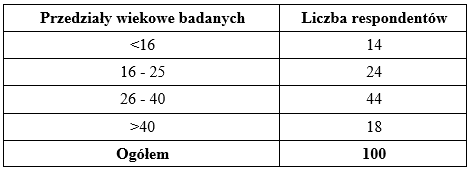
\includegraphics[width=0.75\textwidth]{images/twiek.PNG}
  \caption{Wiek osób biorących udział w badaniu.}
  \caption*{Źródło: opracowanie własne.}
  \label{tbl:twiek}
\end{table}

W tabeli \ref{tbl:twyksztalcenie} zilustrowany jest podział respondentów względem wykształcenia. Najwięcej osób, które udzieliły odpowiedzi posiadają wykształcenie wyższe (54\%). Osoby z wykształceniem średnim i podstawowym stanowią kolejno 26\% oraz 9\%. Pozostałe wykształcenie, opisane jako inne posiadało 11\% badanych.

\clearpage

\begin{table}[htb]
  \centering
  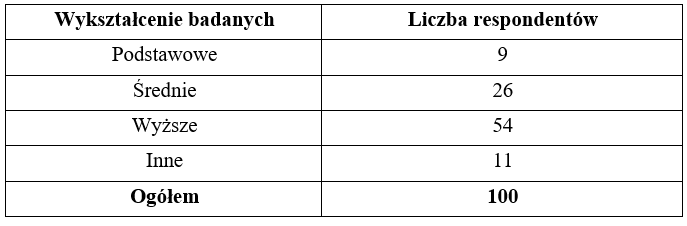
\includegraphics[width=0.85\textwidth]{images/twyksztalcenie.PNG}
  \caption{Wykształcenie osób biorących udział w badaniu.}
  \caption*{Źródło: opracowanie własne.}
  \label{tbl:twyksztalcenie}
\end{table}

Na tym etapie zbadano liczbę osób, które miały doświadczenie z grami VR jak i grami wideo. Odrzuceni zostali respondenci, którzy nie mieli styczności z żadną z platform. Większość z osób, bo aż 93\% korzystało z obu platform, osób korzystających tylko z gier VR było 2\%, a tylko gier wideo 5\%, co ukazuje rysunek \ref{figure:dplatformy}.

\begin{figure}[htb]
  \centering
  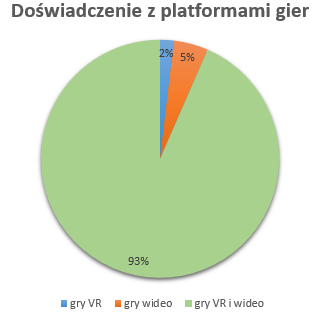
\includegraphics[width=0.6\textwidth]{images/dplatformy.PNG}
  \caption{Doświadczenie z platformami gier osób biorących udział w badaniu.}
  \caption*{Źródło: opracowanie własne.}
  \label{figure:dplatformy}
\end{figure}

\clearpage

\section{Wyniki}

\subsection{Wiek gracza a ulubiona platforma}

Gry wideo jako ulubione medium wybrało 49\% ankietowanych, natomiast gry VR 51\%. Podział ten jednak nie jest tak równomierny w odniesieniu to wieku graczy, co ilustruje rysunek \ref{figure:dwiek}.

\begin{figure}[htb]
  \centering
  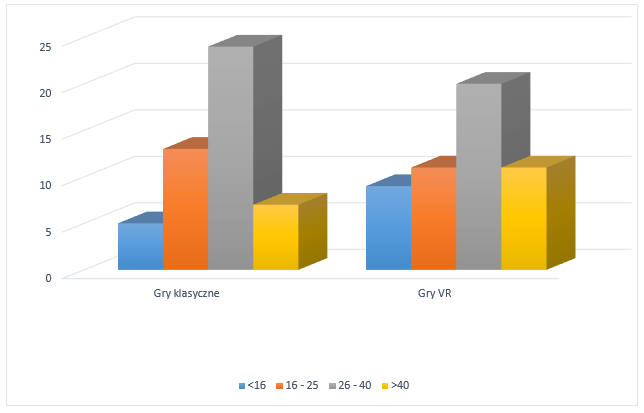
\includegraphics[width=0.9\textwidth]{images/dwiek.PNG}
  \caption{Podział wiekowy użytkowników względem ulubionej platformy.}
  \caption*{Źródło: opracowanie własne.}
  \label{figure:dwiek}
\end{figure}

Z rysunku \ref{figure:dwiek}  wynika, że najmłodsza jak i najstarsza grupa (poniżej 16 oraz powyżej 40 roku życia) badanych preferuje rozgrywkę w trybie VR, natomiast osoby z przedziału wiekowego 16-40 wybierają częściej rozgrywkę w postaci gier wideo. 

\subsection{Czas jednej rozgrywki}

Dane ukazane w tabeli \ref{tbl:tczas} przedstawiają, że czas poświęcony na jedną sesję grania w gry VR, a gry wideo znacząco się różni. W przypadku VR 38\% osób poświęca na grę mniej niż jedną godzinę, a aż 49\% 1 - 2 godzin. Odpowiedź 2 - 5 godzin zaznaczyło 13\%. Żaden z korespondentów nie odpowiedział, że poświęca średnio podczas jednej sesji więcej niż 5 godzin.

Natomiast w przypadku grania w gry wideo, czas poświęcony na jedną sesję, która wynosi mniej niż godzinę to 15\%, a 1 - 2 godzin 33\%. Największy odsetek graczy poświęca na jedną sesję 41\%, a 10\% odpowiadających gra jednorazowo powyżej 5 godzin. 

\clearpage

\begin{table}[htb]
  \centering
  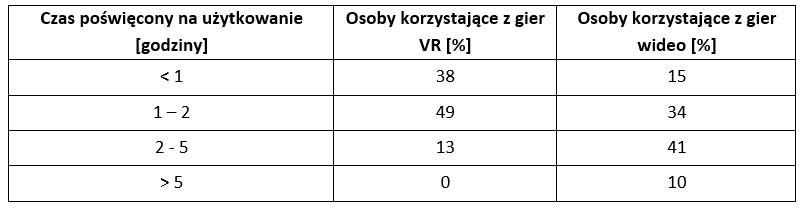
\includegraphics[width=0.8\textwidth]{images/tczas.PNG}
  \caption{Czas poświęcony na użytkowanie przez graczy danej platformy podczas jednej sesji.}
  \caption*{Źródło: opracowanie własne.}
  \label{tbl:tczas}
\end{table}

\subsection{Częstotliwość grania}

Podobna różnorodność jak w przypadku czasu jednej rozgrywki występuje w porównaniu częstotliwości grania w gry VR i gry wideo. Osoby grające rzadziej niż raz w miesiącu stanowią 30\% w przypadku korzystania z technologii VR, oraz 9\% w przypadku korzystania z gier wideo. Wybór przedziału w postaci 1 - 4 razy w miesiącu dokonało kolejno: dla VR 55\%, co było najczęściej wybieraną odpowiedzią, a dla gier wideo 34\%. Kilka razy w tygodniu natomiast z VR korzysta 14\% graczy, a aż 47\% z gier wideo. Najmniej osób odpowiedziało, że gra codziennie w VR (1\%) oraz w gry wideo (11\%).

\begin{table}[htb]
  \centering
  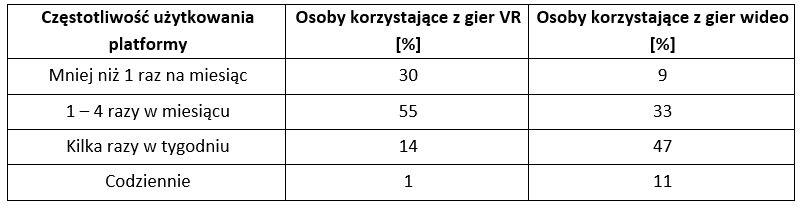
\includegraphics[width=0.9\textwidth]{images/tczestotliwosc.PNG}
  \caption{Częstotliwość użytkowania danej platformy przez graczy.}
  \caption*{Źródło: opracowanie własne.}
  \label{tbl:tczestotliwosc}
\end{table}

\subsection{Immersja a zmęczenie}

Pomimo tego, że respondenci podzielili się na dwie równe grupy jeśli chodzi o preferencje platformy (VR 51\% oraz gry wideo 49\%) to w pytaniach dotyczących wywołania zmęczenia przez grę oraz zdolności gry do pochłonięcia uwagi gracza i wywołania silnych emocji, większość była zgodna. Wyniki tego zestawienia przedstawia tabela \ref{tbl:tzmeczenie}.

\begin{table}[htb]
  \centering
  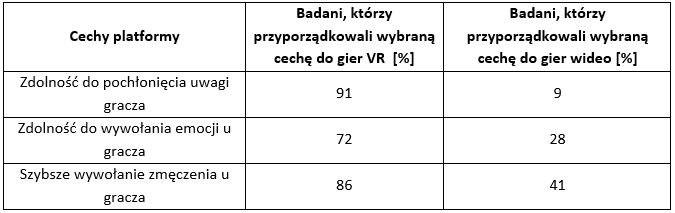
\includegraphics[width=0.9\textwidth]{images/tzmeczenie.PNG}
  \caption{Przyporządkowanie określonych cech do jednej z platform przez ankietowanych.}
  \caption*{Źródło: opracowanie własne.}
  \label{tbl:tzmeczenie}
\end{table}

\subsection{Zdolność platformy do wywołania specyficznych emocji a poziom jej pożądania przez graczy}

Tabela \ref{tbl:tpredyspozycje} wyłania najbardziej i najmniej pożądaną emocję wśród graczy, a także ukazuje predyspozycje gier VR oraz gier wideo do wywołania konkretnych emocji.

\begin{table}[htb]
  \centering
  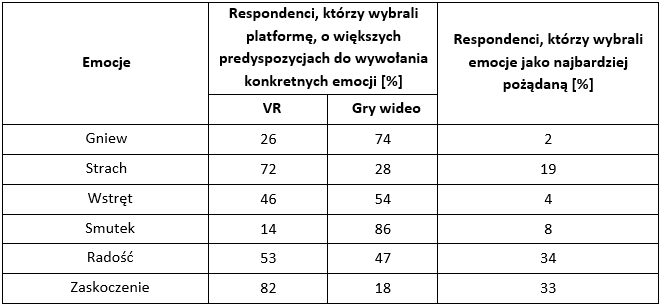
\includegraphics[width=0.8\textwidth]{images/tpredyspozycje.PNG}
  \caption{Emocje i predyspozycje danej platformy do łatwości jej wywołania oraz ważność konkretnej emocji dla graczy.}
  \caption*{Źródło: opracowanie własne.}
  \label{tbl:tpredyspozycje}
\end{table}

Najbardziej pożądaną emocją wśród respondentów okazuje się radość, którą wybrało 34\%. Kolejno były to: zaskoczenie(33\%), strach(19\%), smutek(8\%), wstręt(4\%), gniew(2\%).


Ankietowani wybierali platformę, która ma według nich większe predyspozycje do wywołania konkretnych emocji. Z ankiety wynika, że przy użyciu VR łatwiej wywołać takie emocje jak: zaskoczenie(82\%), strach(72\%) oraz radość(53\%), jednak to gry wideo mają większe predyspozycje do wywołania takich emocji jak: gniew(74\%), wstręt(54\%), smutek(86\%). 

\subsection{Ulubione gatunki gier i ich elementy}

Ulubione gatunki uczestników ankiety przedstawia rysunek \ref{fig:dgatunek}. Większość respondentów za ulubiony gatunek gier wybrało gry zręcznościowe (31\%). Później kolejno: gry sportowe i symulacyjne (29\%), gry przygodowe i fabularne (23\%). Najmniej respondentów uważa za swój ulubiony gatunek gry strategiczne (17\%).

\begin{figure}[htb]
  \centering
  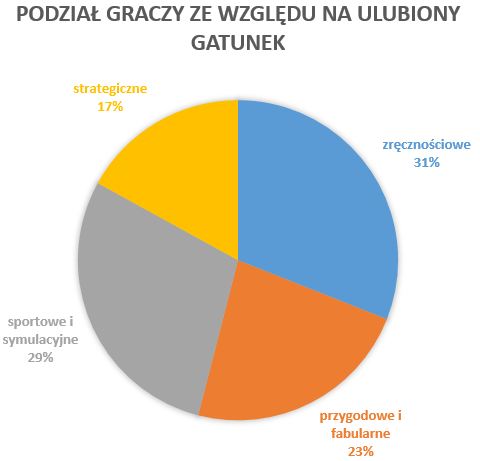
\includegraphics[width=0.8\textwidth]{images/dgatunek.PNG}
  \caption{Ulubione gatunki gier wybrane przez graczy.}
  \caption*{Źródło: opracowanie własne.}
  \label{fig:dgatunek}
\end{figure}

\clearpage

Najbardziej znaczącym elementem rozgrywki dla respondentów okazało się ``wyzwanie, rywalizacja i osiągnięcie sukcesu'' - odpowiedziało tak 43\% ankietowanych, najmniej znaczącym elementem (12\%) zostało ``zaangażowanie ciała w rozgrywkę''. ``doświadczenie społeczne'' oraz ``fabuła, historia, wpływ na jej losy'' są najważniejszym elementem dla podobnej liczby graczy bo kolejno: 22\% i 23\%, co przedstawia tabela \ref{tbl:telementy}.

\begin{table}[htb]
  \centering
  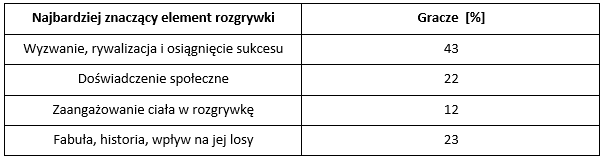
\includegraphics[width=0.8\textwidth]{images/telementy.PNG}
  \caption{Najbardziej znaczące elementy rozgrywki dla graczy.}
  \caption*{Źródło: opracowanie własne.}
  \label{tbl:telementy}
\end{table}

\subsection{Wady i zalety obu platform}

Respondenci w pytaniach otwartych udzielili odpowiedzi na pytanie jakie są wady i zalety obu platform. Na podstawie najczęściej występujących odpowiedzi stworzona została tabela  \ref{tbl:twadyzalety}.

\begin{table}[htb]
  \centering
  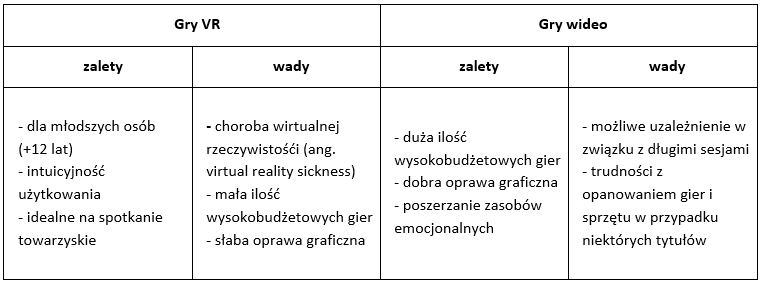
\includegraphics[width=1\textwidth]{images/twadyzalety.PNG}
  \caption{Najczęściej wymieniane wady i zalety gier VR i gier wideo przez respondentów.}
  \caption*{Źródło: opracowanie własne.}
  \label{tbl:twadyzalety}
\end{table}

   

% WNIOSKI !!!!!!!!!!!!!!!!!!!!!!!!!!!!!!!!!
    
    
\section{Wnioski}

\subsection{Preferencje graczy}

Analizując dane na temat wieku oraz preferencji co do ulubionej platformy, zauważalny jest znaczny podział na dwie grupy. Osoby najmłodsze jak i najstarsze preferują rozgrywkę w formie VR, natomiast osoby w wieku 16-40 wybierają gry wideo. Dane z ankiety pochodzą z roku 2020, więc osoby te urodziły się w latach 1980-2004. Spora część osób będących w tym przedziale swoją młodość spędzała w latach, kiedy dużą popularnością cieszyły się gry arcade, gry komputerowe oraz konsolowe, czyli te występujące po tzw. złotej erze gier arcade - lata 80,90 XX wieku oraz na początku XXI wieku.  Można wywnioskować, że osoby te miały styczność z grami w latach młodości, co pozwoliło im na obycie się z różnego typu sprzętem i wyrobiło pewne umiejętności, które przydają się w erze dzisiejszych gier wideo. Kolejną kwestią może być przyzwyczajenie użytkowników do tego typu gier. Osoby młode, czyli te poniżej 16 lat oraz osoby powyżej 40 lat mogły nie mieć okazji aby zainteresować się grami wideo. Można zauważyć, że te osoby często wybierają rozrywkę w trybie VR lub tą, dostarczaną przez urządzenia mobilne - głównie telefony typu smartfon. Potwierdzają to także odpowiedzi w pytaniach otwartych, gdzie jedną z częściej wymienianych zalet VR jest intuicyjność. Próg wejścia dla młodych graczy oraz starszych osób jeśli chodzi o gry wideo nie jest tak niski jak w przypadku gier VR.

Osoby korzystające z obu platform najczęściej wybierają gry zręcznościowe, sportowe oraz symulacyjne, a większość ankietowanych wybrało ``Wyzwanie, rywalizację i osiągnięcie sukcesu'' jako najbardziej znaczący element rozgrywki. Dowodzi to, że osoby korzystające zarówno z VR jak i gier wideo mają podobne preferencje co do gatunku gier, jak i cenią w grach podobne elementy rozgrywki. Ma to związek z tym, że gry VR polegają najczęściej na rywalizacji poprzez proste czynności, lecz bez skomplikowanej fabuły. Na podstawie danych z tabeli \ref{tbl:twadyzalety} można stwierdzić, że gry VR najczęściej wybierane są ze względu na intuicyjność, prostotę oraz formę zabawy, przeciwstawnie do gier wideo, gdzie gracze głównie oczekują rozbudowanej rozgrywki z dobrą oprawą graficzną. Można wysnuć wniosek, że preferencje graczy znacznie się różnią - część z nich zależy od konkretnych cech użytkownika, inne natomiast to kwestia zainteresowań lub upodobań.


\subsection{Charakter rozgrywki}

VR charakteryzuje się dużą zdolnością do wywołania emocji oraz bardzo łatwo pochłania uwagę gracza. Analizując dane wykryto zależność między kilkoma czynnikami:
\begin{itemize}
  \item zdolnością VR do pochłonięcia uwagi gracza,
  \item zdolnością VR do wywołania emocji,
  \item częstotliwością grania,
  \item czasem grania.
\end{itemize}

Spoglądając na dane, można stwierdzić, że osoby korzystające z VR najczęściej poświęcają na grę maksymalnie 2 godziny podczas jednej sesji, która odbywa się od 1 do 4 razy w miesiącu. Inny charakter ma korzystanie z gier wideo - kiedy to pojedyncza sesja trwa najczęściej od 2 do 5 godzin i jest odbywana kilka razy w tygodniu. Analizując te dane można zauważyć pewną zależność - zdolność gier do dużej immersji prowadzi do wywołania silnych emocji, co z kolei negatywnie skutkuje zmęczeniem fizycznym oraz psychicznym po krótkiej rozgrywce, dlatego osoby sięgają po gry VR rzadziej jak i na krótszy czas. Gry wideo z kolei są mniej męczące, bardziej komfortowe i pozwalają na częstszą i dłuższą rozgrywkę. Gry wideo z reguły dostarczają mniej intensywnych przeżyć niż gry VR, ale pozwalają na większy relaks i odpoczynek. 

\subsection{Predyspozycje platform do wywołania specyficznych emocji u użytkownika}

%OLD  

% Zarówno gry VR jak i gry wideo są dobrym sposobem na wywołanie emocji u swoich użytkowników. Większość z ankietowanych odpowiedziało, że zdolność gier do wywołania określonych stanów emocjonalnych jest dla nich bardzo ważna. VR dzięki swoim cechom ma dużą zdolność do wywołania emocji podczas rozgrywek lecz ze względu na początkowe stadium rozwoju tej technologii w porównaniu do gier wideo nie ma ona tak dużo zwolenników. Z ankiety wynika, że to VR ma większe predyspozycje do wywołania najbardziej pożądanych emocji przez graczy (radość, zaskoczenie, strach) lecz nie jest tak popularną formą rozrywki jak gry wideo. Aktualne liczbę graczy ogółem na świecie szacuje się na ponad 2.5 miliarda, z czego gracze VR to tylko 171 milionów\citep{website:gameindustry, website:vrstats}. Liczba ta ciągle rośnie, a to za sprawą wciąż rozwijającej się technologii VR. Największą zmorą VR jest brak "pełnoprawnych" gier, lecz i to ulega zmianie. Wydanie jednej, dobrze przyjętej przez graczy produkcji może znacząco zmienić liczbę aktywnych graczy. Przykładem może być wydanie gry "Half-Life: Alyx", kiedy  w ciągu jednego miesiąca odnotowano przyrost 1 miliona nowych użytkowników VR\citep{website:alyx}.

%  NEW

% Technologia VR pozwala na wywołanie silnych i intensywnych emocji u swoich
% użytkowników, lecz niesie to za sobą także negatywne skutki, stad wiele osób wybiera
% klasyczne gry wideo. Zestawiając obie formy użytkowania gier (tj. wideo i VR) oraz biorąc
% pod uwagę emocjonalność gracza możemy wyodrębnić wiele zalet i wad, które wpływają na
% wywoływanie danego afektu u użytkownika. Wybór platformy zależy w głównej mierze od
% tego, jakiego rodzaju rozrywki oczekuje użytkownik. Intensywność wywołanych emocji, ich
% nacechowanie oraz sposób rozgrywki znacząco się różni w przypadku obu platform stąd
% porównywanie, która z nich jest lepsza wydaje się być bezcelowe. Gry VR często występują
% w nieskomplikowanych formach, aniżeli jako pełnoprawny produkt konsumencki. Jednym z
% wyjątków jest wymieniony wielokrotnie w pracy ‘Half Life Alyx’, który można nazwać
% faktyczną pełnoprawną wersją gry VR. Jak zostało opisane w tekście, każda forma wpływa na
% inny rodzaj emocji. Tak samo postrzegają to ankietowani, wg których znaczną przewagę nad
% wywoływaniem m.in. zaskoczenia ma technologia VR.

%  NEW NEW

Zarówno gry VR jak i gry wideo są dobrym sposobem na wywołanie emocji u swoich użytkowników. Większość z ankietowanych odpowiedziało, że zdolność gier do wywołania określonych stanów emocjonalnych jest dla nich bardzo ważna. Najbardziej pożądanymi emocjami są kolejno: radość, zaskoczenie i strach. Najmniej natomiast: gniew wstręt oraz smutek. 

VR dzięki swoim cechom ma dużą zdolność do wywołania emocji podczas rozgrywek lecz ze względu na początkowe stadium rozwoju tej technologii w porównaniu do gier wideo nie ma ona tak dużo zwolenników. Technologia VR pozwala na wywołanie silnych i intensywnych emocji u swoich
użytkowników, lecz niesie to za sobą także negatywne skutki (zmęczenie psychiczne i fizyczne oraz symptomy choroby wirtualnej rzeczywistości - podobne do choroby lokomocyjnej), stąd wiele osób wybiera klasyczne gry wideo.

Z ankiety wynika, że to VR ma większe predyspozycje do wywołania najbardziej pożądanych emocji przez graczy (radość, zaskoczenie, strach) lecz nie jest tak popularną formą rozrywki jak gry wideo. Zauważyć więc można związek między platformą a rodzajem emocji które wywołuje. VR znacząco lepiej radzi sobie z wywołaniem zaskoczenia oraz strachu w porównaniu do gier wideo, które z kolei lepiej radzą sobie z wywołaniem smutku u graczy. Predyspozycje platform do wywołania radości i wstrętu są bardzo zbliżone, natomiast większość badanych wybrało gry wideo jako platformę mającą większą zdolność do wywołania gniewu. Analizując dane wywnioskować można, że chociaż nie wszystkie emocje są nacechowane pozytywnie, są one pożądane przez graczy. Tymi, które są najważniejsze dla graczy to kolejno: radość, zaskoczenie i strach, a te najmniej pożądane to gniew wstręt oraz smutek. Na podstawie analizy można wywnioskować, że wywołanie emocji przez gry jest pożądane z perspektywy gracza oraz można stwierdzić, że każda z platform operuje specyficznymi zdolnościami do wywołania określonych emocji. 


% % STARE !!!!!!!!!!!!!!!!!!!!!!

% \subsection{Cechy gracza}

% Analizując dane na temat wieku oraz preferencji co do ulubionej platformy, zauważalny jest znaczny podział na dwie grupy. Osoby najmłodsze jak i najstarsze preferują rozgrywkę w formie VR, natomiast osoby w wieku 16-40 wybierają gry wideo. Dane z ankiety pochodzą z roku 2020, więc osoby te urodziły się w latach 1980-2004. Spora część osób będących w tym przedziale swoją młodość spędzała w latach, kiedy dużą popularnością cieszyły się gry arcade, gry komputerowe oraz konsolowe, czyli te występujące po tzw. złotej erze gier arcade - lata 80,90 XX wieku oraz 00 XXI wieku.  Można wywnioskować, że osoby te miały styczność z grami w latach młodości, co pozwoliło im na obycie się z różnego typu sprzętem i wyrobiło pewne umiejętności, które przydają się w erze dzisiejszych gier wideo. Kolejną kwestią może być przyzwyczajenie użytkowników do tego typu gier. Osoby młode, czyli te poniżej 16 lat oraz osoby powyżej 40 lat mogły nie mieć okazji aby zainteresować się grami wideo. Można zauważyć, że te osoby często wybierają rozrywkę w trybie VR lub tą, dostarczaną przez urządzenia mobilne - głównie telefony typu smartfon. Potwierdzają to także odpowiedzi w pytaniach otwartych, gdzie jedną z częściej wymienianych zalet VR jest intuicyjność. Próg wejścia dla młodych graczy oraz starszych osób jeśli chodzi o gry wideo nie jest tak niski jak w przypadku gier VR.


% \subsection{Immersja}

% VR charakteryzuje się dużą zdolnością do wywołania emocji oraz bardzo łatwo pochłania uwagę gracza. Analizując dane wykryto zależność między kilkoma czynikami:

% \begin{itemize}
%   \item zdolnością VR do wywołania emocji,
%   \item częstotliwością grania,
%   \item czasem grania.
% \end{itemize}

% Spoglądając na dane, można stwierdzić, że osoby korzystające z VR najczęściej poświęcają na grę maksymalnie 2 godziny podczas jednej sesji, która odbywa się od 1 do 4 razy w miesiącu. Inny charakter ma korzystanie z gier wideo - kiedy to pojedyncza sesja trwa najczęściej od 2 do 5 godzin, i jest odbywana kilka razy w tygodniu. Analizując te dane można zauważyć pewną zależność - zdolność gier do dużej immersji prowadzi do wywołania silnych emocji, co z kolei negatywnie skutkuje zmeczęniem fizycznym oraz psychicznym po krótkiej rozgrywce dlatego osoby sięgają po gry VR rzadziej jak i na krótszy czas. Gry wideo z kolei są mniej męczące, bardziej komfortowe i pozwalają na częstszą i dłuższą rozgrywkę. Gry wideo z reguły dostarczają mniej intensywnych przeżyć niż gry VR ale pozwala to na większy relaks i odpoczynek. 


% \subsection{Emocje jako czynnik sukcesu}

% Zarówno gry VR jak i gry wideo są dobrym sposobem na wywołanie emocji u swoich użytkowników.VR dzięki swoim cechom ma dużą zdolność do wywołania emocji podczas rozgrywek lecz ze względu na początkowe stadium rozwoju tej technologii w porównaniu do gier wideo nie ma ona tak dużo zwolenników. Z ankiety wynika, że to VR ma większe predyspozycje do wywołania najbardziej pożądanych emocji przez graczy (z reguły tych pozytywnych) lecz nie jest tak popularną formą rozrywki jak gry wideo. Większość z ankietowanych odpowiedziało, że zdolność gier do wywołania określonych stanów emocjonalnych jest dla nich ważna lub najważniejsza.

% Aktualne liczbę graczy ogółem na świecie szacuje się na ponad 2.5 miliarda, z czego gracze VR to tylko 171 milionów\citep{website:gameindustry, website:vrstats}. Liczba ta ciągle rośnie, a to za sprawą wciąż rozwijającej się technologii VR. Największą zmorą VR jest brak "pełnoprawnych" gier, lecz i to ulega zmianie. Wydanie jednej, dobrze przyjętej przez graczy produkcji może znacząco zmienić liczbę aktywnych graczy. Przykładem może być wydanie gry "Half-Life: Alyx", kiedy  w ciągu jednego miesiąca odnotowano przyrost 1 miliona nowych użytkowników VR\citep{website:alyx}.

% \subsection{Preferencje użytkownika a wybór platformy}

% Granie w gry VR znacząco rózni się od klasycznej rozgrywki. Na podstawie najczęściej występujących odpowiedzi badanych na temat wad i zalet obu platform stworzona została tabela zaprezentowana poniżej.

% \begin{table}[htb]
%   \centering
%   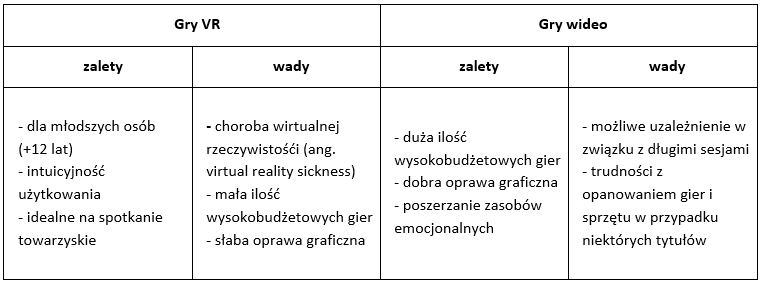
\includegraphics[width=0.8\textwidth]{images/twadyzalety.PNG}
%   \caption{Najczęściej wymieniane wady i zalety przez ankietowanych}
%   \caption*{Źródło: opracowanie własne}
%   \label{tbl:twadyzalety}
% \end{table}

% % Wybór platformy i gatunku gier zależy w głównej mierze od tego, jakiego rodzaju rozrywki oczekuje użytkownik. Intensywność wywołanych emocji, ich nacechowanie oraz sposób rozgrywki znacząco się różni w przypadku obu platform stąd porównywanie, która z nich jest lepsza wydaje się być bezcelowym. Gry wideo mają inny charakter niż gry VR, które z kolei po pewnym czasie stają się męczące i monotonne - polegają najczęsciej na prostych czynnościach, bez skompliokwanaje fabuły. Rynek VR wciąż ewoluuje i producenci gier coraz częściej będą tworzyć coraz bardziej zaawansowane dzieła, czego przykładem może być wcześniej wymieniony "Half-Life: Alyx".
